\documentclass[11pt]{article}

% ---------------------------------------------------------------------------
% Packages
% ---------------------------------------------------------------------------
\usepackage[a4paper,margin=2.4cm]{geometry}
\usepackage[utf8]{inputenc}
\usepackage[T1]{fontenc}
\usepackage{amsmath,amssymb,amsfonts}
\usepackage{graphicx}
\usepackage{xcolor}
\usepackage{booktabs}
\usepackage{longtable}
\usepackage{array}
\usepackage{enumitem}
\usepackage{caption}
\usepackage{listings}
\usepackage{tikz}
\usetikzlibrary{arrows.meta,positioning,fit,backgrounds,shapes.geometric,calc}
\usepackage{fancyhdr}
\usepackage{titlesec}
\usepackage[colorlinks=true,linkcolor=blue!50!black,citecolor=blue!50!black,urlcolor=blue!50!black,bookmarksopen=true]{hyperref}
\usepackage{parskip}
\usepackage{float}
\usepackage[framemethod=default]{mdframed}

% ---------------------------------------------------------------------------
% Colors
% ---------------------------------------------------------------------------
\definecolor{codebg}{RGB}{246,248,250}
\definecolor{codeframe}{RGB}{210,214,220}
\definecolor{kwcolor}{RGB}{175,40,40}
\definecolor{strcolor}{RGB}{30,110,40}
\definecolor{cmtcolor}{RGB}{110,110,110}
\definecolor{numcolor}{RGB}{30,80,160}
\definecolor{boxblue}{RGB}{235,242,250}
\definecolor{boxgreen}{RGB}{233,246,238}
\definecolor{boxamber}{RGB}{252,244,228}
\definecolor{boxgray}{RGB}{240,240,240}
\definecolor{boxviolet}{RGB}{240,235,250}

% ---------------------------------------------------------------------------
% Listings style (Python)
% ---------------------------------------------------------------------------
\lstdefinestyle{py}{
  language=Python,
  backgroundcolor=\color{codebg},
  rulecolor=\color{codeframe},
  frame=single,
  framerule=0.4pt,
  basicstyle=\ttfamily\footnotesize,
  keywordstyle=\color{kwcolor}\bfseries,
  stringstyle=\color{strcolor},
  commentstyle=\color{cmtcolor}\itshape,
  numberstyle=\tiny\color{numcolor},
  numbers=left,
  numbersep=8pt,
  showstringspaces=false,
  breaklines=true,
  breakatwhitespace=false,
  tabsize=4,
  columns=fullflexible,
  captionpos=b,
  xleftmargin=1.2em,
  xrightmargin=0.2em,
  aboveskip=8pt,
  belowskip=6pt,
}
\lstset{style=py}

\newcommand{\srcref}[1]{\hfill\textcolor{cmtcolor}{\footnotesize\texttt{#1}}}
\newcommand{\code}[1]{\texttt{\small #1}}

% ---------------------------------------------------------------------------
% Rationale / decision boxes (mdframed - properly balanced environments)
% ---------------------------------------------------------------------------
\mdfdefinestyle{calloutbase}{
  linewidth=0pt, innertopmargin=6pt, innerbottommargin=6pt,
  innerleftmargin=8pt, innerrightmargin=8pt,
  skipabove=8pt, skipbelow=8pt, roundcorner=3pt,
}
\newmdenv[style=calloutbase, backgroundcolor=boxblue]{rationale}
\newmdenv[style=calloutbase, backgroundcolor=boxgray]{dims}
\newmdenv[style=calloutbase, backgroundcolor=boxamber]{optional}
\newmdenv[style=calloutbase, backgroundcolor=boxviolet]{fixnote}

\newcommand{\rationalelabel}{\small\textbf{Rationale.}~}
\newcommand{\dimslabel}{\small\textbf{Tensor shapes.}~}
\newcommand{\optionallabel}{\small\textbf{Optional component (opt-in, default off).}~}
\newcommand{\fixnotelabel}{\small\textbf{Implementation note.}~}

% ---------------------------------------------------------------------------
% Header/footer
% ---------------------------------------------------------------------------
\pagestyle{fancy}
\fancyhf{}
\fancyhead[L]{\small FX Direction Prediction \& Risk-Parity Overlay --- Methodology}
\fancyhead[R]{\small\thepage}
\renewcommand{\headrulewidth}{0.3pt}

\titleformat{\section}{\normalfont\Large\bfseries}{\thesection}{0.6em}{}
\titleformat{\subsection}{\normalfont\large\bfseries}{\thesubsection}{0.6em}{}
\titleformat{\subsubsection}{\normalfont\bfseries}{\thesubsubsection}{0.6em}{}

\title{\vspace{-1.5cm}\textbf{Methodology: Independent Per-Asset FX Direction Prediction\\ with a Risk-Parity Portfolio Overlay}\\[6pt]
\large Architecture, Mathematical Formulation, and Implementation Reference}
\author{Repository: \texttt{mlforecasting} \\ Modules: \texttt{models/portfolio\_lstm.py}, \texttt{models/portfolio\_pnl.py}, \texttt{api/server.py}}
\date{\today}

\begin{document}
\maketitle
\thispagestyle{empty}

\begin{abstract}
\noindent
This document describes, in full mathematical and implementation detail, an FX
direction-prediction and portfolio-construction system. $N$ \textbf{fully independent}
per-asset LSTMs (\texttt{AssetLSTM}, one per FX pair, no shared weights, no shared
optimizer), each followed by a \textbf{causal self-attention} layer over the lookback
window, map a rolling window of cross-sectional log-return-derived features to a
heteroscedastic $(\mu,\sigma)$ pair at every day in the window. Training minimizes a
Gaussian negative log-likelihood plus a direction-matching binary cross-entropy term, per
asset, with no gradient ever crossing between assets unless an optional
\texttt{cross\_pairs} link widens what one asset's network \emph{reads} (never what
\emph{optimizes} it). A calibrated directional probability is recovered via the probit
link, and a configurable \emph{neutral band} lets the model abstain on samples with
insufficient edge. Downstream, an evaluation-only \textbf{risk-parity portfolio overlay}
(\texttt{models/portfolio\_pnl.py}) converts each asset's probability into a signal,
weights it by an equal-risk-contribution solve over a rolling covariance estimate, smooths
it over the model's own forecast horizon, and scales the book to a target annualized
volatility -- reported alongside an unmodulated risk-parity baseline. An
\textbf{optional complementary training objective} lets this same portfolio Sharpe ratio
feed back into training itself, in a second, genuinely joint phase layered on top of the
otherwise-independent per-asset optimization. Every architectural choice is presented
alongside its rationale, the governing mathematical expression, the exact source file and
line range implementing it, and a worked numerical example. The document closes with a
full results section training three progressively richer model configurations on three
FX pairs chosen for cross-sectional diversification (EUR, JPY, and AUD legs against USD),
a complete configuration reference, and a summary of every architectural decision and its
motivation.
\end{abstract}

\vspace{0.3cm}
\tableofcontents
\newpage

% =============================================================================
\section{Notation and Conventions}
\label{sec:notation}
% =============================================================================

\begin{center}
\renewcommand{\arraystretch}{1.25}
\begin{tabular}{@{}cll@{}}
\toprule
\textbf{Symbol} & \textbf{Code name} & \textbf{Meaning} \\
\midrule
$N$ & \texttt{n\_assets} & Number of tradable FX pairs \\
$L$ & \texttt{lookback} & Sequence length: trailing days in one input window \\
$C$ & \texttt{n\_channels} & Feature channels PER PAIR (depends on the selected feature set, \S\ref{sec:features}) \\
$H$ & \texttt{hidden\_size} & Each \texttt{AssetLSTM}'s LSTM hidden state width \\
$B$ & (implicit) & Number of decision samples in a split (full-batch training, no minibatching) \\
$K$ & \texttt{n\_attn\_heads} & Attention heads in each asset's causal self-attention layer \\
$H_{\text{d}}$ & \texttt{direction\_horizon} & Forward days the z-score label looks (default 5) \\
$W_{\text{r}}$ & \texttt{rolling\_stats\_window} & Trailing window for rolling vol/skew/kurtosis features + label normalization (default 20) \\
$W_{\text{c}}$ & \texttt{cov\_window} & Trailing window for the portfolio overlay's rolling covariance (default 60) \\
\bottomrule
\end{tabular}
\end{center}

A raw daily log return is $r_t \in \mathbb{R}^N$. The full asset-major feature block for
one decision sample is $X_i \in \mathbb{R}^{L \times NC}$ (\S\ref{sec:features}); a full
split's worth is a rank-3 tensor $X \in \mathbb{R}^{B \times L \times NC}$. Superscript
``raw'' denotes a pre-standardization quantity; a hat ($\hat{\cdot}$) denotes a model
estimate. All neural network code is PyTorch; every \code{nn.LSTM} is instantiated with
\code{batch\_first=True}. Training is \textbf{full-batch}: one epoch is one forward/backward
pass over the entire training split at once, never a shuffled minibatch loop -- this is not
merely an implementation detail but a load-bearing assumption for the optional Sharpe
training objective in \S\ref{sec:sharpeobjective}, which needs its samples in chronological
order.

Every feature/behavior described below that is \textbf{off by default} is marked with an
\textbf{Optional component} box; Section~\ref{sec:config} tabulates every configuration key
and its default.

% =============================================================================
\section{System Overview}
\label{sec:overview}
% =============================================================================

The system has two structurally different stages that are trained \textbf{never jointly by
default}: (1) \texttt{PredictionModel}, $N$ independent \texttt{AssetLSTM} networks, each
predicting its own asset's forward direction; and (2) an evaluation-time (or, optionally,
also training-time -- \S\ref{sec:sharpeobjective}) \textbf{risk-parity portfolio overlay}
that turns those $N$ independent probabilities into a single book of position sizes.

\begin{enumerate}[label=\textbf{Stage \arabic*.}, leftmargin=2.2cm]
  \item \textbf{Data \& features} (\S\ref{sec:data}): daily close prices $\to$ log returns
    $\to$ a configurable per-pair feature set (raw return, rolling vol/skew/kurtosis, FX
    carry, moving-average crossover, causal Butterworth band-pass) $\to$ rolling windows
    $\to$ chronological train/validation/test split with purge/embargo $\to$
    train-only standardization.
  \item \textbf{\texttt{AssetLSTM}} (\S\ref{sec:assetlstm}): $N$ independent LSTM + causal
    self-attention networks, one per pair, each reading the FULL cross-sectional feature
    block (or a configurable subset of other pairs' blocks via \texttt{cross\_pairs|}) and
    outputting a dense, per-day heteroscedastic $(\mu,\sigma)$ pair.
  \item \textbf{Training} (\S\ref{sec:training}): each asset's own \texttt{torch.optim.Adam}
    instance minimizes Gaussian NLL + a direction BCE term, computed from \emph{only that
    asset's own} output and label -- fully independent, verified empirically
    (\S\ref{sec:verification}). An optional second, genuinely \emph{joint} phase
    (\S\ref{sec:sharpeobjective}) can add a portfolio-Sharpe objective on top.
  \item \textbf{Calibration \& reporting} (\S\ref{sec:calibration}--\ref{sec:neutralband}):
    a validation-fit residual-scale correction $\hat\sigma_{\text{hat}}$, the probit link to
    a calibrated probability, a neutral band for abstention, and the standard
    confusion-matrix metrics.
  \item \textbf{Portfolio overlay} (\S\ref{sec:portfolio}): each asset's probability becomes
    a signal in $[-1,1]$, weighted by an equal-risk-contribution solve, smoothed over the
    model's own forecast horizon, and scaled to a target annualized volatility -- reported
    against an unmodulated risk-parity baseline.
\end{enumerate}

\begin{figure}[H]
\centering
\resizebox{\textwidth}{!}{%
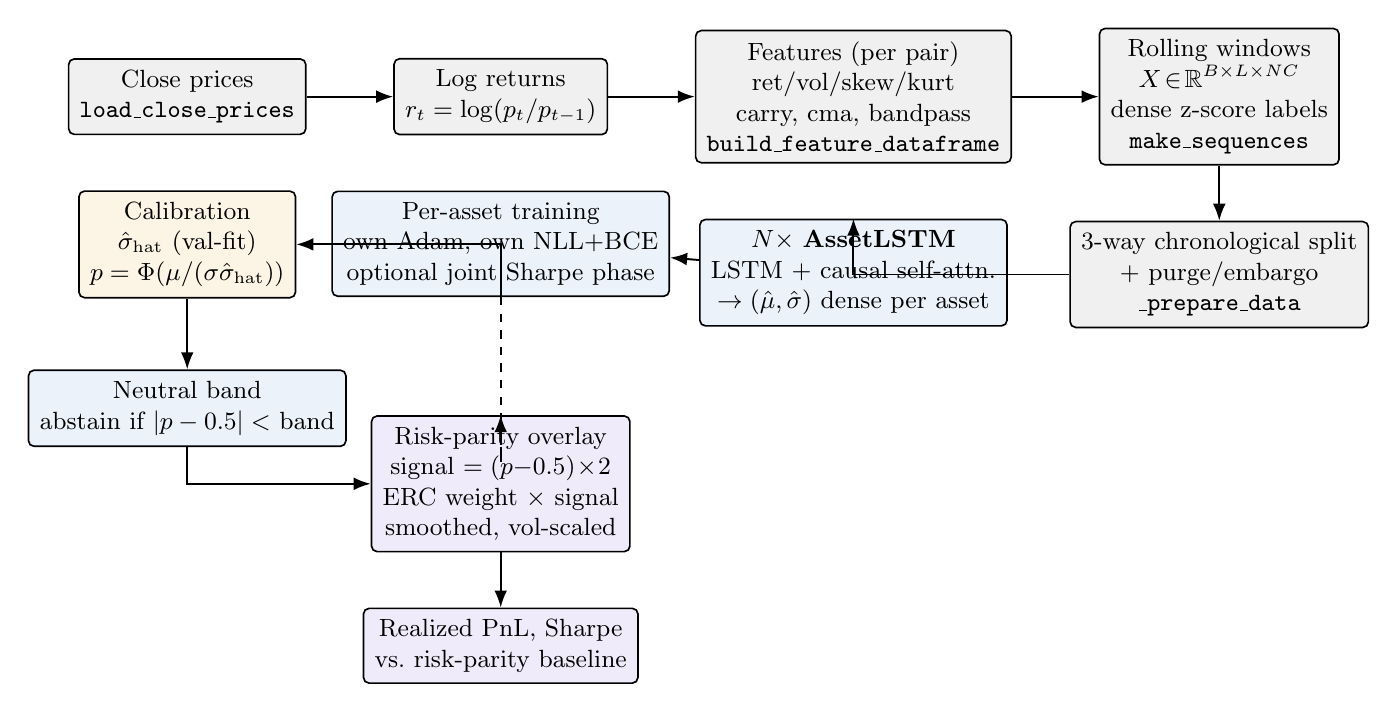
\begin{tikzpicture}[
  node distance=7mm and 11mm,
  every node/.style={font=\small},
  box/.style={draw, rounded corners=2pt, minimum height=9mm, align=center, inner sep=4pt, line width=0.6pt},
  data/.style={box, fill=boxgray},
  net/.style={box, fill=boxblue},
  risk/.style={box, fill=boxamber},
  bench/.style={box, fill=boxviolet},
  opt/.style={dashed},
  arr/.style={-Latex, line width=0.7pt}
]
\node[data] (prices) {Close prices\\ \texttt{load\_close\_prices}};
\node[data, right=of prices] (returns) {Log returns\\ $r_t = \log(p_t/p_{t-1})$};
\node[data, right=of returns] (features) {Features (per pair)\\ ret/vol/skew/kurt\\ carry, cma, bandpass\\ \texttt{build\_feature\_dataframe}};
\node[data, right=of features] (windows) {Rolling windows\\ $X\!\in\!\mathbb{R}^{B\times L\times NC}$\\ dense z-score labels\\ \texttt{make\_sequences}};
\node[data, below=of windows] (split) {3-way chronological split\\ + purge/embargo\\ \texttt{\_prepare\_data}};

\node[net, below=of features] (assetlstm) {$N \times$ \textbf{AssetLSTM}\\ LSTM + causal self-attn.\\ $\to (\hat\mu,\hat\sigma)$ dense per asset};
\node[net, below=of returns] (train) {Per-asset training\\ own Adam, own NLL+BCE\\ optional joint Sharpe phase};

\node[risk, below=of prices, xshift=-0mm] (calib) {Calibration\\ $\hat\sigma_{\text{hat}}$ (val-fit)\\ $p=\Phi(\mu/(\sigma\hat\sigma_{\text{hat}}))$};
\node[net, below=of calib, yshift=-2mm] (band) {Neutral band\\ abstain if $|p-0.5|<$ band};

\node[bench, below=of train, yshift=-8mm] (overlay) {Risk-parity overlay\\ signal $=(p{-}0.5)\!\times\!2$\\ ERC weight $\times$ signal\\ smoothed, vol-scaled};
\node[bench, below=of overlay] (pnl) {Realized PnL, Sharpe\\ vs.\ risk-parity baseline};

\draw[arr] (prices) -- (returns);
\draw[arr] (returns) -- (features);
\draw[arr] (features) -- (windows);
\draw[arr] (windows) -- (split);
\draw[arr] (split.west) -| (assetlstm.north);
\draw[arr] (assetlstm) -- (train);
\draw[arr] (train.south) |- (calib.east);
\draw[arr] (calib) -- (band);
\draw[arr] (band) |- (overlay);
\draw[arr, opt] (train.south) |- ([yshift=-6mm]overlay.north) -- (overlay.north);
\draw[arr] (overlay) -- (pnl);
\end{tikzpicture}%
}
\caption{End-to-end pipeline. Dashed arrow: the optional joint Sharpe training phase
(\S\ref{sec:sharpeobjective}) reuses the SAME risk-parity overlay machinery inside training
itself, not just at evaluation time. Grey = data/feature engineering, blue = per-asset
prediction, amber = calibration/reporting, violet = portfolio overlay.}
\label{fig:pipeline}
\end{figure}

\begin{rationale}\rationalelabel
Per-asset independence is the load-bearing design decision of the whole prediction stage:
each asset's own gradient magnitude, Adam's per-parameter adaptive state, and which epoch its
own checkpoint gets restored from depend on nothing but that asset's own loss curve,
regardless of how many other assets are being trained alongside it. This was verified
\emph{empirically}, not just by inspection: \texttt{smoke\_test.py} trains an asset "A" solo
versus alongside an unrelated pure-noise asset "B" (same seed, \texttt{dropout=0}) and asserts
byte-identical hit rates (\S\ref{sec:verification}) -- observed result: \texttt{0.485} versus
\texttt{0.485}, exactly. The portfolio overlay is the one place cross-asset information is
genuinely combined, and even there, by default, it is pure \emph{postprocessing}: it never
touches the weights that produced the probabilities it consumes, unless the optional Sharpe
objective (\S\ref{sec:sharpeobjective}) is explicitly turned on -- and even then, only that
one additional phase becomes joint; the primary NLL+BCE phase remains untouched.
\end{rationale}

% =============================================================================
\section{Data Pipeline and Feature Engineering}
\label{sec:data}
% =============================================================================

\subsection{Price loading and log returns}

\begin{lstlisting}[caption={Close prices from Postgres, downloading/upserting on demand.}, label=lst:loadclose]
def load_close_prices(symbols: list[str], years: int) -> pd.DataFrame:
    end = date.today()
    start = end - timedelta(days=365 * years)
    prices = get_time_series(symbols, start, end)
    missing = [s for s in symbols if s not in prices.columns or prices[s].dropna().empty]
    if missing:
        downloader = FXDownloader(years=years)
        fresh = {s: downloader.download_pair(s, MAJOR_FX_PAIRS.get(s, f"{s}=X")) for s in missing}
        upsert_pairs(fresh)
        prices = get_time_series(symbols, start, end)
    return prices.dropna()   # inner-join on date

def to_log_returns(prices: pd.DataFrame) -> pd.DataFrame:
    return np.log(prices / prices.shift(1)).dropna()
\end{lstlisting}
\srcref{models/portfolio\_lstm.py:197--229}

\begin{equation}
  r_t = \log\!\left(\frac{p_t}{p_{t-1}}\right) \in \mathbb{R}^N
  \label{eq:logret}
\end{equation}

\begin{rationale}\rationalelabel
Log returns are additive across time ($\sum_t r_t = \log(p_T/p_0)$), which every downstream
variance/covariance computation (the rolling moments in \S\ref{sec:features}, the portfolio
overlay's covariance in \S\ref{sec:riskparity}) implicitly assumes. Prices are inner-joined
(\code{dropna()}) across every requested pair so every downstream window is defined on
exactly the same calendar days for every asset -- a single stale/missing quote for one pair
would otherwise silently misalign that day's cross-sectional feature block.
\end{rationale}

\subsection{The feature catalog}
\label{sec:features}

Every per-pair input channel this system knows how to build is enumerated in a single,
fixed-order catalog:

\begin{lstlisting}[caption={The fixed feature catalog and its defaults.}, label=lst:catalog]
FEATURE_CATALOG: tuple[str, ...] = ("log_return", "vol", "skew", "kurt", "carry", "cma", "bandpass")
DEFAULT_FEATURES: list[str] = ["log_return", "vol", "skew", "kurt"]
DEFAULT_CMA_WINDOWS: list[tuple[int, int]] = [[10, 50]]
DEFAULT_BANDPASS_WINDOWS: list[tuple[int, int]] = [[10, 50]]
DEFAULT_BANDPASS_ORDER: int = 3
\end{lstlisting}
\srcref{models/portfolio\_lstm.py:301--327}

A caller's \code{features} list is a \emph{selection} out of this catalog, never an
ordering directive -- columns are always assembled in the catalog's own fixed order, per
pair, asset-major (all of one pair's channels contiguous, then the next pair's):
\begin{equation}
  X_i = \big[\, \underbrace{r^{(1)}, \text{vol}^{(1)}, \dots}_{\text{pair }1,\ C\text{ channels}},\;
               \underbrace{r^{(2)}, \dots}_{\text{pair }2},\; \dots \,\big] \in \mathbb{R}^{L\times NC}
  \label{eq:assetmajor}
\end{equation}
\code{"cma"} and \code{"bandpass"} are special: each contributes \emph{one channel per
window pair} in \code{cma\_windows}/\code{bandpass\_windows}, not one channel total:
\begin{equation}
  C = \underbrace{\big|\{f \in \text{features} : f \notin \{\text{cma},\text{bandpass}\}\}\big|}_{\text{base features}}
    + \underbrace{|\text{cma\_windows}| \cdot \mathbb{1}[\text{cma}\in\text{features}]}_{\text{cma channels}}
    + \underbrace{|\text{bandpass\_windows}| \cdot \mathbb{1}[\text{bandpass}\in\text{features}]}_{\text{bandpass channels}}
  \label{eq:nchannels}
\end{equation}
\srcref{models/portfolio\_lstm.py:330--346 (\texttt{n\_channels\_per\_pair})}

\paragraph{(a) Raw log return.} Channel 0 whenever \code{"log\_return"} is selected: $r_t$
itself, Equation~\ref{eq:logret}.

\paragraph{(b/c/d) Rolling moments: volatility, skewness, excess kurtosis.}
\begin{equation}
  \text{vol}_t = \mathrm{std}(r_{t-W_r+1},\dots,r_t), \quad
  \text{skew}_t = \mathrm{skew}(r_{t-W_r+1},\dots,r_t), \quad
  \text{kurt}_t = \mathrm{kurt}(r_{t-W_r+1},\dots,r_t) - 3
  \label{eq:moments}
\end{equation}
(pandas' \code{.kurt()} already subtracts 3, i.e.\ \emph{excess} kurtosis, so a Gaussian
series reports $\approx 0$). $W_r = $ \texttt{rolling\_stats\_window} (default 20) is the
SAME window that normalizes the forward z-score label (\S\ref{sec:labels}), so the label's
scale matches what the model can itself observe about recent volatility.
\srcref{models/portfolio\_lstm.py:276--298 (\texttt{rolling\_moment\_features})}

\paragraph{(e) Carry (interest-rate differential).}
\begin{equation}
  \text{carry}_t^{(b,q)} = \frac{\rho_t^{(b)} - \rho_t^{(q)}}{100}
  \label{eq:carry}
\end{equation}
for a pair with base currency $b$ and quote currency $q$ (e.g.\ \texttt{EURUSD}
$\Rightarrow b{=}$EUR, $q{=}$USD), where $\rho_t^{(c)}$ is currency $c$'s short-term policy
rate (FRED, monthly) at time $t$. Reindexed onto the daily index with
\textbf{forward-fill only} -- never back-filled, so no future rate print leaks backward; any
day before the first available print is $0$.
\begin{lstlisting}[caption={Carry: forward-fill only, never back-filled.}, label=lst:carry]
diff = (rates[base] - rates[quote]) / 100.0
carry[pair] = diff.reindex(carry.index, method="ffill").fillna(0.0)
\end{lstlisting}
\srcref{models/portfolio\_lstm.py:239--273 (\texttt{load\_carry})}

\paragraph{(f) Cross moving averages (trend).} For each \code{(short, long)} window pair:
\begin{equation}
  \text{cma}_t^{(s,l)} = \overline{r}_{t}^{(s)} - \overline{r}_{t}^{(l)}, \qquad
  \overline{r}_t^{(w)} = \frac{1}{w}\sum_{k=0}^{w-1} r_{t-k}
  \label{eq:cma}
\end{equation}
positive when the recent (short-window) trend runs above the longer-run (long-window)
trend -- the return-space analogue of a classic price moving-average crossover. Purely
trailing (\code{min\_periods=window}, no back-fill).
\srcref{models/portfolio\_lstm.py:349--376 (\texttt{cross\_moving\_averages})}

\paragraph{(g) Causal Butterworth band-pass (faster-reacting trend).} An SMA-difference
(Eq.~\ref{eq:cma}) is a crude, high-lag approximation of a band-pass filter. A genuine
Butterworth design achieves comparable noise rejection with markedly less phase lag. For a
$(\text{short\_period}, \text{long\_period})$ pair in \emph{days}, the passband (in cycles/day,
Nyquist $= 0.5$ for once-daily-sampled data) is
\begin{equation}
  f_{\text{low}} = \frac{1/\text{long\_period}}{0.5}, \qquad
  f_{\text{high}} = \frac{1/\text{short\_period}}{0.5}, \qquad
  0 < f_{\text{low}} < f_{\text{high}} < 1
  \label{eq:bandedges}
\end{equation}
(\texttt{short\_period} sets the high cutoff -- the fastest cycle length that still passes;
\texttt{long\_period} sets the low cutoff, removing the long-run trend/DC component). The
filter's transfer function $H(z) = B(z)/A(z)$ (numerator/denominator polynomials of order
\texttt{order}, default 3) is obtained from a standard analog Butterworth prototype via the
bilinear transform (\texttt{scipy.signal.butter}), and applied via the direct-form-II
transposed difference equation
\begin{equation}
  a_0 y_t = \sum_{k=0}^{P} b_k\, r_{t-k} \;-\; \sum_{k=1}^{P} a_k\, y_{t-k}
  \label{eq:lfilter}
\end{equation}
($P = 2\!\times\!\texttt{order}$ for a band-pass filter) -- i.e.\ \texttt{scipy.signal.lfilter},
\textbf{forward-only}.

\begin{lstlisting}[caption={Causal Butterworth band-pass - \texttt{lfilter}, deliberately NOT \texttt{filtfilt}.}, label=lst:bandpass]
from scipy.signal import butter, lfilter
nyquist = 0.5
low  = (1.0 / long_period) / nyquist
high = (1.0 / short_period) / nyquist
b, a = butter(order, [low, high], btype="bandpass")
filtered = lfilter(b, a, returns[pair].to_numpy(dtype=np.float64))
series.iloc[:long_period] = np.nan   # filter transient hasn't settled yet
\end{lstlisting}
\srcref{models/portfolio\_lstm.py:379--442 (\texttt{butterworth\_bandpass\_features})}

\begin{rationale}\rationalelabel
\texttt{scipy.signal.filtfilt} is the \emph{usual} way a Butterworth filter is applied (it
runs the filter forward, then backward, canceling phase distortion entirely) -- but the
backward pass uses samples \emph{after} the point being filtered, which is non-causal and
would leak future returns into today's feature value, exactly the look-ahead leakage the
rest of this pipeline (purge/embargo, trailing-only rolling features, the causal attention
mask in \S\ref{sec:assetlstm}) is built to avoid. \texttt{lfilter} keeps every output
strictly a function of past and current samples, at the cost of some unavoidable phase lag
-- a genuinely causal filter can never fully cancel it. It is still empirically faster to
react than a CMA crossover for comparable noise rejection (\S\ref{sec:verification},
smoke\_test.py test 8c: peaks 5 days after a synthetic regime shift, versus a CMA
crossover's 9 days), because a proper Butterworth design shapes its passband/stopband far
more efficiently than differencing two plain moving averages.
\end{rationale}

\begin{fixnote}\fixnotelabel
\textbf{Numerical stability of the IIR recursion.} Equation~\ref{eq:lfilter} is an
infinite-impulse-response recursion; for a very low \texttt{long\_period} cutoff (poles
close to the unit circle), the direct \texttt{(b, a)} transfer-function form can be
numerically sensitive to coefficient rounding at high order. This was investigated directly
against this project's own real FX history (8 years, 7 major pairs) for
\texttt{bandpass\_windows}$=[[5,25],[50,100]]$: no NaN/Inf beyond the intentional
\texttt{long\_period}-row transient-masking region were observed, so the current
\texttt{(b, a)} + \texttt{lfilter} implementation was kept as-is; a second-order-sections
(\texttt{output="sos"}) form is the standard, more conservative alternative if a future,
more extreme window combination were ever found to be unstable.
\end{fixnote}

\paragraph{Assembly and NaN handling.} All selected channels are assembled asset-major
(Eq.~\ref{eq:assetmajor}) into one wide DataFrame, then forward-filled and any still-leading
NaN (not enough trailing history for the very first rows) is set to a neutral $0.0$ --
\textbf{never back-filled}, which would leak a later value into an earlier row:
\begin{lstlisting}[caption={Feature assembly - one function builds every selected channel.}, label=lst:buildfeat]
features_df = features_df.ffill().fillna(0.0)
assert features_df.shape[1] == n_channels_per_pair(features, cma_windows, bandpass_windows) * len(pairs)
\end{lstlisting}
\srcref{models/portfolio\_lstm.py:445--502 (\texttt{build\_feature\_dataframe})}

\subsection{Standardization}

Per-feature mean/std are fit \textbf{only on the training split} and reused, unchanged, for
validation and test (and, when loading a saved model, restored from its checkpoint rather
than refit):
\begin{equation}
  \mu = \mathrm{mean}_{(B,L)}\big(X^{\text{train,raw}}\big),\qquad
  \sigma = \mathrm{std}_{(B,L)}\big(X^{\text{train,raw}}\big) + 10^{-8},\qquad
  X^{\text{split}} = \frac{X^{\text{split,raw}} - \mu}{\sigma}
  \label{eq:standardize}
\end{equation}
\srcref{models/portfolio\_lstm.py:505--507 (\texttt{standardize}), 1954--1960 (\texttt{\_prepare\_data})}

% =============================================================================
\section{Sequence Construction and Labels}
\label{sec:labels}
% =============================================================================

\subsection{The forward z-score label}

For each pair, the label is the \textbf{forward, direction\_horizon-day cumulative return},
expressed in trailing-volatility standard deviations:
\begin{equation}
  z_d = \frac{\sum_{k=1}^{H_d} r_{d+k}}{\text{vol}_d \cdot \sqrt{H_d}}
  \label{eq:zlabel}
\end{equation}
where $\text{vol}_d$ is the SAME trailing rolling volatility used as an input feature
(Eq.~\ref{eq:moments}) -- known as of day $d$'s close, no look-ahead -- and the $\sqrt{H_d}$
scaling is the standard i.i.d.-returns assumption that an $H_d$-day sum's standard deviation
scales as the daily standard deviation times $\sqrt{H_d}$. This keeps each move's
\emph{magnitude}, not just its sign, and normalizes it consistently with the volatility
input feature so a 1\% move on a quiet pair and a 3\% move on a volatile one can land at a
similar z-score if both are equally "surprising" relative to their own recent volatility.
\begin{lstlisting}[caption={Vectorized forward z-score label via a cumulative-sum trick.}, label=lst:zlabel]
padded_cumsum = np.concatenate([np.zeros((1, n)), np.cumsum(values, axis=0)], axis=0)
forward_sum = padded_cumsum[H+1 : valid+H+1] - padded_cumsum[1 : valid+1]
z[:valid] = forward_sum / (trailing_vol[:valid] * np.sqrt(H) + eps)
\end{lstlisting}
\srcref{models/portfolio\_lstm.py:510--544 (\texttt{\_forward\_zscore\_labels})}

\begin{rationale}\rationalelabel
$\text{sign}(z_d)$ is exactly the realized direction -- what hit rate/confusion matrices use
-- but the CONTINUOUS magnitude is what \texttt{AssetLSTM} is actually supervised against
(as the mean of a Gaussian, \S\ref{sec:losses}): a pure classification label throws away
information about how confidently a given day's move should be predicted, which a proper
scoring rule like Gaussian NLL can use to calibrate $\sigma$ per sample.
\end{rationale}

\subsection{Dense, per-day supervision within each window}

\begin{lstlisting}[caption={Sliding window construction - X, next-day returns, and DENSE per-day labels.}, label=lst:makeseq]
for start in range(first_start, last_start):
    day_t = start + lookback - 1                 # the decision day
    X.append(feature_values[start : day_t + 1])            # (L, NC)
    next_returns.append(values[day_t + 1])                   # (N,) - raw, for PnL only
    z_labels.append(full_z[start : day_t + 1])               # (L, N) - one label PER DAY in the window
    dates.append(index[day_t + 1])
\end{lstlisting}
\srcref{models/portfolio\_lstm.py:547--623 (\texttt{make\_sequences})}

Crucially, \code{z\_labels[i]} carries \textbf{one label per day inside the window}, not
just at the decision day: window sample $i$'s label at position $k$ is pair $p$'s own
$H_d$-day-forward z-score computed as of window-day $k$ -- entirely a function of days
\emph{after} $k$, so supervising every position in the window is never look-ahead leakage,
merely "does everything computable at day $k$'s close accurately predict day $k$'s own
forward outcome", repeated for every $k$. \texttt{next\_returns[i]}, by contrast, is the
single \emph{raw}, un-featurized return realized the day after the window -- used only for
realized-PnL reporting (\S\ref{sec:portfolio}), never as a training target.

\begin{dims}\dimslabel
$X \in \mathbb{R}^{B\times L\times NC}$; \code{next\_returns} $\in \mathbb{R}^{B\times N}$;
\code{z\_labels} $\in \mathbb{R}^{B \times L \times N}$ (dense).
\end{dims}

\subsection{Chronological split, and purge/embargo at each boundary}
\label{sec:split}

The split is strictly chronological -- the most recent \code{test\_frac} fraction of all
samples is carved off \emph{first} as test, then \code{train\_frac} splits whatever remains:
\begin{align}
  n_{\text{test}} &= \lfloor n_{\text{total}} \cdot \texttt{test\_frac} \rfloor, &
  n_{\text{remaining}} &= n_{\text{total}} - n_{\text{test}}, &
  n_{\text{train}} &= \lfloor n_{\text{remaining}} \cdot \texttt{train\_frac} \rfloor
\end{align}
Because consecutive samples are stride-1, a sample's forward label window and its lookback
input window overlap heavily with its neighbors' -- right at a split boundary this would let
information the model was trained to predict leak into what the next split "sees" as recent
history. \code{purge\_gap} $= L + H_d$ samples are dropped \emph{entirely} (not reassigned)
at each boundary that genuinely separates two non-empty splits:
\begin{lstlisting}[caption={Purge/embargo - only at a boundary that actually separates two splits.}, label=lst:purge]
purge_gap = lookback + direction_horizon
train_end = max(n_train - purge_gap, 0) if n_train < n_remaining else n_train
val_end   = max(n_remaining - purge_gap, n_train) if n_test > 0 else n_remaining
\end{lstlisting}
\srcref{models/portfolio\_lstm.py:1902--1952 (\texttt{\_prepare\_data})}

\begin{fixnote}\fixnotelabel
\textbf{The conditional guards matter.} An earlier version purged \code{train\_end}/
\code{val\_end} unconditionally. This is correct whenever \texttt{train\_frac}$<1$ (training
mode: there really is a validation split after train, and a test split after that), but
\textbf{evaluation mode} (the API's \code{/api/evaluate} endpoint) deliberately sets
\texttt{train\_frac}$=1.0$, \texttt{test\_frac}$=0.0$ so the WHOLE fetched period is one
continuous evaluation block. With the unconditional version, purging would still trim
\code{purge\_gap} ($\approx 35$) days off the \emph{end} of that block even though there is
no downstream split left to protect from leakage -- needlessly discarding the freshest,
most valuable days for no reason. The guards above (\code{n\_train < n\_remaining},
\code{n\_test > 0}) make purging conditional on a boundary actually existing.
\end{fixnote}

% =============================================================================
\section{\texttt{AssetLSTM}: One Asset's Independent Predictor}
\label{sec:assetlstm}
% =============================================================================

Each pair gets its own dedicated \texttt{AssetLSTM} -- \textbf{no parameters shared with any
other asset}. Its \emph{input}, however, can be the full cross-sectional feature block (or a
configurable subset -- \S\ref{sec:crosspairs}), so its recurrence can still react to another
pair's same-day move without a separate cross-asset stage or the bottleneck of only seeing a
compressed summary of it.

\begin{figure}[H]
\centering
\resizebox{0.92\textwidth}{!}{%
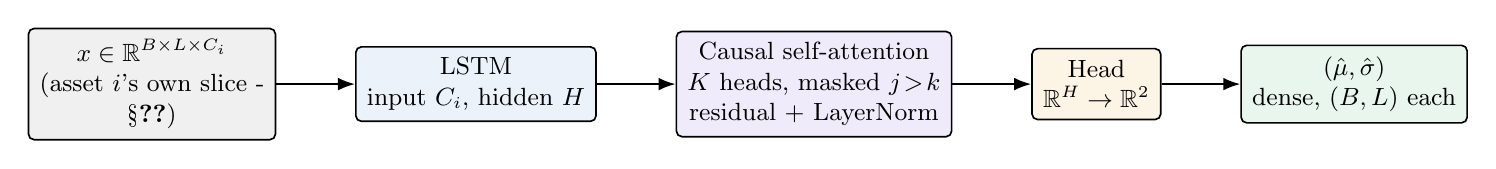
\begin{tikzpicture}[
  node distance=7mm and 10mm,
  every node/.style={font=\small},
  box/.style={draw, rounded corners=2pt, minimum height=9mm, align=center, inner sep=4pt, line width=0.6pt},
  inbox/.style={box, fill=boxgray},
  lstmbox/.style={box, fill=boxblue},
  attn/.style={box, fill=boxviolet},
  headbox/.style={box, fill=boxamber},
  arr/.style={-Latex, line width=0.7pt}
]
\node[inbox] (x) {$x \in \mathbb{R}^{B\times L\times C_i}$\\ (asset $i$'s own slice -\\ \S\ref{sec:crosspairs})};
\node[lstmbox, right=of x] (lstm) {LSTM\\ input $C_i$, hidden $H$};
\node[attn, right=of lstm] (attn) {Causal self-attention\\ $K$ heads, masked $j\!>\!k$\\ residual + LayerNorm};
\node[headbox, right=of attn] (head) {Head\\ $\mathbb{R}^H \to \mathbb{R}^2$};
\node[box, fill=boxgreen, right=of head] (out) {$(\hat\mu, \hat\sigma)$\\ dense, $(B,L)$ each};

\draw[arr] (x) -- (lstm);
\draw[arr] (lstm) -- (attn);
\draw[arr] (attn) -- (head);
\draw[arr] (head) -- (out);
\end{tikzpicture}%
}
\caption{One \texttt{AssetLSTM}. Every pair gets an independently-parameterized instance of
this exact block; only the input width $C_i = |\text{included\_indices}_i| \times C$ can
differ (\S\ref{sec:crosspairs}).}
\label{fig:assetlstm}
\end{figure}

\begin{lstlisting}[caption={AssetLSTM: LSTM, causal self-attention, heteroscedastic head.}, label=lst:assetlstm]
class AssetLSTM(nn.Module):
    def __init__(self, input_size, hidden_size=16, num_layers=1, dropout=0.0, n_attn_heads=4):
        self.lstm = nn.LSTM(input_size, hidden_size, num_layers, batch_first=True)
        self.attn = nn.MultiheadAttention(hidden_size, n_attn_heads, dropout=dropout, batch_first=True)
        self.attn_norm = nn.LayerNorm(hidden_size)
        self.head = nn.Linear(hidden_size, 2)
        with torch.no_grad():
            self.head.bias[1].fill_(0.5413)   # softplus(0.5413) = 1.0 -> sigma ~= 1 at init

    def forward(self, x):                                     # x: (B, L, input_size)
        lstm_out, _ = self.lstm(x)                              # (B, L, H)
        lookback = lstm_out.shape[1]
        causal_mask = torch.triu(torch.full((lookback, lookback), float("-inf")), diagonal=1)
        attn_out, _ = self.attn(lstm_out, lstm_out, lstm_out, attn_mask=causal_mask, need_weights=False)
        h = self.attn_norm(lstm_out + attn_out)                 # residual + LayerNorm
        out = self.head(h)                                      # (B, L, 2)
        mu = out[..., 0]
        sigma = F.softplus(out[..., 1]) + 1e-3
        return mu, sigma
\end{lstlisting}
\srcref{models/portfolio\_lstm.py:630--724}

\subsection{Causal self-attention}

The LSTM's hidden state at day $k$ already summarizes $x_{0..k}$ recurrently, but that
summary is a fixed-size bottleneck. Self-attention lets day $k$'s representation pull
directly from any \emph{earlier} day's hidden state:
\begin{equation}
  \text{Attn}(Q,K,V) = \mathrm{softmax}\!\left(\frac{QK^\top}{\sqrt{d_k}} + M\right) V, \qquad
  M_{jk} = \begin{cases} 0 & j \le k \\ -\infty & j > k \end{cases}
  \label{eq:causalattn}
\end{equation}
with $Q=K=V=\text{lstm\_out}$ (self-attention) and $M$ the upper-triangular causal mask
(Eq.~\ref{eq:causalattn}, \code{torch.triu(..., diagonal=1)}). The mask is \textbf{mandatory}:
this network outputs a prediction at every day in the window, each one supervised as if
computed using only information through that day (\S\ref{sec:labels}); an unmasked
(bidirectional) attention layer would let day $k$'s prediction see days after $k$ -- exactly
the label look-ahead leakage the rest of this pipeline is built to avoid. Implemented as a
residual block (post-norm Transformer pattern), so early in training, before the attention
weights have learned anything useful, the LSTM's own signal still passes through unchanged:
\begin{equation}
  h = \mathrm{LayerNorm}\big(\text{lstm\_out} + \text{Attn}(\text{lstm\_out})\big)
  \label{eq:residual}
\end{equation}

\begin{rationale}\rationalelabel
\textbf{Empirically verified, not just asserted}: \texttt{smoke\_test.py} test 1b perturbs
only the LAST timestep of a window and confirms every EARLIER day's prediction is
byte-identical before and after (\code{torch.allclose(mu\_a[:, :-1, :], mu\_b[:, :-1, :])})
while the last day's own prediction DOES change -- direct proof the mask is doing its job,
not merely present in the code.
\end{rationale}

\subsection{The heteroscedastic head}

\begin{equation}
  \hat\mu_{i,k} \in \mathbb{R} \ \text{(unbounded)}, \qquad
  \hat\sigma_{i,k} = \mathrm{softplus}(\text{out}_{i,k,1}) + 10^{-3} \ \text{(strictly positive)}
  \label{eq:heterosced}
\end{equation}
The head's sigma-half bias is initialized so $\mathrm{softplus}(\text{bias}) \approx 1.0$ --
the network starts out claiming predictive std $=1$ (the label's own unconditional scale),
i.e.\ $p \approx \Phi(\hat\mu) \approx 0.5$ while $\hat\mu$ is still near its own small random
init -- a calibrated-ignorance starting point rather than random over/under-confidence the
network must first unlearn.

\begin{fixnote}\fixnotelabel
\textbf{The $10^{-3}$ floor matters for a different, real reason.} If $\hat\sigma$ is driven
toward $0$ by a large-capacity network overfitting a single sample's residual early in
training, both \texttt{gaussian\_nll} (Eq.~\ref{eq:nll}) and \texttt{direction\_bce}
(Eq.~\ref{eq:bce}) divide by $\sigma$ -- an unbounded-below NLL surface as
$\sigma\!\to\!0^+$. The floor bounds $1/\sigma$ at $1000$; this does NOT, by itself, prevent
exploding gradients on a sufficiently large/deep architecture -- see the documented
\texttt{device="mps"} + \texttt{num\_layers}$>$1 numerical issue in
\S\ref{sec:numericalissues}, discovered via exactly this failure mode.
\end{fixnote}

% =============================================================================
\section{\texttt{PredictionModel}: $N$ Assets as One Persistable Unit}
\label{sec:predictionmodel}
% =============================================================================

\texttt{PredictionModel} owns $N$ \texttt{AssetLSTM} instances (\code{nn.ModuleList}) purely
as a persistence/inference convenience -- \code{forward()} runs every asset for batched
inference, but \S\ref{sec:training} shows training never actually calls this combined
\code{forward()}.

\subsection{\texttt{cross\_pairs}: opt-in, per-pair input widening}
\label{sec:crosspairs}

\begin{optional}\optionallabel
\texttt{cross\_pairs} (default \code{\{\}}) is a \code{\{pair: [other\_pair, ...]\}} dict.
DEFAULT: every pair's own LSTM sees \emph{only} its own $C$-channel block -- fully
independent, no cross-asset mixing at all. A pair listed as a key gets its OWN features
(always included) plus every listed other pair's FULL feature block.
\end{optional}

\begin{lstlisting}[caption={Building each asset's own input-slice indices.}, label=lst:crosspairs]
pair_index = {p: i for i, p in enumerate(self.pairs)}
self.included_indices = []
for pair in self.pairs:
    ordered = [pair] + [p for p in self.cross_pairs.get(pair, []) if p != pair]
    indices = [pair_index[p] for p in dict.fromkeys(ordered)]   # de-duplicated, own pair first
    self.included_indices.append(indices)

self.assets = nn.ModuleList([
    AssetLSTM(len(indices) * n_channels, hidden_size, num_layers, dropout, n_attn_heads)
    for indices in self.included_indices
])
\end{lstlisting}
\srcref{models/portfolio\_lstm.py:786--822}

\begin{equation}
  C_i = |\text{included\_indices}_i| \cdot C, \qquad
  \text{asset\_input}(x, i) = \big[\, x_{:,:,\,\text{idx}\cdot C : (\text{idx}+1)\cdot C} \,\big]_{\text{idx}\,\in\,\text{included\_indices}_i}
  \label{eq:assetinput}
\end{equation}
Unknown pairs referenced in \texttt{cross\_pairs} raise a \code{ValueError} immediately
(construction time), rather than silently being ignored.

\begin{rationale}\rationalelabel
This replaced an earlier design where \emph{every} asset unconditionally saw \emph{every}
pair's features -- unconditional full mixing had the same bottleneck-avoidance goal but no
way to dial it back down when it wasn't paying for itself on a given pair. \texttt{cross\_pairs}
makes cross-asset information flow a per-pair, explicit, opt-in choice, with "fully
independent" as the honest default. Verified (\S\ref{sec:verification}, smoke\_test.py test
1a): by default \code{included\_indices == [[0], [1], [2]]} for 3 pairs; linking one pair to
the other two widens ONLY that pair's own input, e.g.\ \code{[[0,1,2], [1], [2]]}.
\end{rationale}

% =============================================================================
\section{Loss Functions}
\label{sec:losses}
% =============================================================================

\subsection{Gaussian negative log-likelihood}

\begin{equation}
  \mathcal{L}_{\text{NLL}}(\mu,\sigma,z) = \frac{1}{BL}\sum_{i,k} \frac{1}{2}\Big(2\log\sigma_{i,k} + \Big(\frac{z_{i,k}-\mu_{i,k}}{\sigma_{i,k}}\Big)^{\!2}\Big)
  \label{eq:nll}
\end{equation}
\begin{lstlisting}[caption={Gaussian NLL - the constant $\log 2\pi$ term is dropped (doesn't affect gradients).}, label=lst:nll]
def gaussian_nll(mu, sigma, target):
    return (0.5 * (2.0 * torch.log(sigma) + ((target - mu) / sigma) ** 2)).mean()
\end{lstlisting}
\srcref{models/portfolio\_lstm.py:1034--1045}

The proper scoring rule for a heteroscedastic $(\mu,\sigma)$ head: unlike a plain
point-estimate loss, the model can LOWER its loss on unpredictable samples by RAISING
$\sigma$ there (an honest "I don't know", $p\to 0.5$) while keeping $\sigma$ small -- and
getting full credit -- on samples where $\mu$ genuinely discriminates.

\subsection{The direction anti-collapse term}

A bare regression loss (Eq.~\ref{eq:nll} alone) is minimized by $\mu \to \mathbb{E}[z]$ -- one
constant sign for every sample whenever the target is barely predictable, i.e.\ the
degenerate all-recall/zero-specificity confusion matrix. The BCE term is instead minimized
by matching each SAMPLE's own sign:
\begin{equation}
  p_{i,k} = \Phi(\mu_{i,k} / \sigma_{i,k}), \qquad
  \mathcal{L}_{\text{BCE}} = -\frac{1}{BL}\sum_{i,k} \Big[ y_{i,k}\log p_{i,k} + (1-y_{i,k})\log(1-p_{i,k}) \Big], \quad y_{i,k}=\mathbb{1}[z_{i,k}>0]
  \label{eq:bce}
\end{equation}
\begin{lstlisting}[caption={Direction BCE, via ndtr (NOT log\_ndtr - see the note below).}, label=lst:bce]
def direction_bce(mu, sigma, target_z):
    score = mu / sigma
    y = (target_z > 0).to(score.dtype)
    log_p     = torch.log(torch.clamp(torch.special.ndtr(score),  min=1e-12))
    log_not_p = torch.log(torch.clamp(torch.special.ndtr(-score), min=1e-12))
    return -(y * log_p + (1.0 - y) * log_not_p).mean()
\end{lstlisting}
\srcref{models/portfolio\_lstm.py:1048--1077}

The total per-asset loss is $\mathcal{L} = \mathcal{L}_{\text{NLL}} + \lambda_{\text{bce}}
\mathcal{L}_{\text{BCE}}$ (\code{bce\_weight} $\lambda_{\text{bce}}$, default $1.0$; $0$
recovers pure distributional regression, collapse risk and all). Where nothing in the
features discriminates, the BCE optimum is exactly $p = $ base rate $\approx 0.5$, which the
neutral band (\S\ref{sec:neutralband}) then reports as an honest abstention rather than a
coin-flip call.

\begin{fixnote}\fixnotelabel
\textbf{Why \texttt{ndtr}, not \texttt{log\_ndtr}.} \code{torch.special.log\_ndtr} is
numerically nicer (avoids materializing a probability that could round to exactly 0 or 1),
but is \textbf{not implemented on the MPS backend} as of this codebase's target PyTorch
version -- and this runs every single training epoch. Reaching for it would force a
CPU-fallback environment variable on every call rather than running natively on Apple
Silicon's Metal backend. The \code{clamp(min=1e-12)} floor only ever binds for
astronomically extreme/miscalibrated scores, far outside anything a z-score head trained
under Eq.~\ref{eq:nll} actually produces. This exact substitution (\code{ndtr} instead of
\code{log\_ndtr}) is itself the fix for a real MPS \code{NotImplementedError} hit earlier in
this project's development.
\end{fixnote}

\subsection{The probit link}

\begin{equation}
  \Phi(z) = P(\mathcal{N}(0,1) \le z), \qquad p = \Phi\!\left(\frac{\mu}{\sigma\,\hat\sigma_{\text{hat}}}\right)
  \label{eq:probit}
\end{equation}
\code{torch.special.ndtr} -- the standard normal CDF, recovering a calibrated probability
from a continuous z-score. $z=0$ maps to exactly $0.5$, so every downstream threshold-at-0.5
consumer (hit rate, confusion matrix) agrees exactly with $\mathrm{sign}(z)$.
\srcref{models/portfolio\_lstm.py:1011--1031 (\texttt{probit})}

% =============================================================================
\section{Training: Fully Independent per Asset}
\label{sec:training}
% =============================================================================

Every asset gets its OWN \code{torch.optim.Adam} instance (own momentum/variance state,
entirely separate from every other asset's) and its OWN loss, computed from just that
asset's own $(\mu,\sigma)$ and label:
\begin{lstlisting}[caption={Per-asset training loop - own optimizer, own loss, own backward/step.}, label=lst:trainloop]
optimizers = [torch.optim.Adam(model.assets[i].parameters(), lr=lr, weight_decay=weight_decay)
              for i in range(n_assets)]
for epoch in range(1, epochs + 1):
    for i in range(n_assets):
        optimizers[i].zero_grad()
        x_i = model.asset_input(X_train, i)
        mu_i, sigma_i = model.assets[i](x_i)                     # (n_train, lookback)
        target_i = z_labels_train[:, :, i]
        loss_i = gaussian_nll(mu_i, sigma_i, target_i) + bce_weight * direction_bce(mu_i, sigma_i, target_i)
        loss_i.backward()
        _assert_finite_grad(model.assets[i].parameters(), f"epoch {epoch}, asset {i}")
        optimizers[i].step()
\end{lstlisting}
\srcref{models/portfolio\_lstm.py:1304--1479 (\texttt{train\_prediction\_model})}

Applied to the FULL dense $(B,L)$ output for that asset -- not just the window's last day --
since every day in every window is its own supervised sample (\S\ref{sec:labels}), and
because consecutive windows slide by one day, a given calendar day is trained on repeatedly
(once per window it falls inside) rather than just once, with no need to separately
up-weight it.

\begin{rationale}\rationalelabel
Nothing about how asset $i$ trains -- gradient magnitude, Adam's per-parameter adaptive
state, which epoch its checkpoint gets restored from -- depends on how many OTHER assets are
being trained alongside it, or how they are doing. An asset linked to another pair's
features via \texttt{cross\_pairs} still trains this way: cross\_pairs only widens what its
LSTM READS, never what optimizes it. \textbf{Empirically verified}
(\S\ref{sec:verification}, smoke\_test.py test 1c): asset "A" trained solo reports hit rate
$0.485$; the SAME asset "A" trained alongside an unrelated pure-noise asset "B" (same seed,
\code{dropout=0} to remove an RNG-interleaving confound) also reports $0.485$ -- bit-for-bit
identical.
\end{rationale}

\subsection{Per-asset checkpoint selection}

If a validation split is tracked, the SAME per-asset loss -- but on the decision day only,
matching what is actually reported -- is computed after every epoch, and each asset's OWN
best-epoch state dict is restored independently at the end:
\begin{lstlisting}[caption={Per-asset validation tracking and independent checkpoint restoration.}, label=lst:checkpoint]
if val_loss_i < best_val_loss[i]:
    best_val_loss[i] = val_loss_i
    best_state[i] = copy.deepcopy(model.assets[i].state_dict())
...
for i in range(n_assets):
    model.assets[i].load_state_dict(best_state[i])   # each asset's OWN best epoch
\end{lstlisting}
\srcref{models/portfolio\_lstm.py:1413--1423, 1498--1524}

Deliberately \emph{not} selected on validation hit rate: hit rate is a coarse, saturating
metric (once every sample's sign is correct it cannot improve further no matter how much more
confident/well-calibrated the predictions get), so selecting on it tends to freeze onto
whichever epoch first reached its ceiling -- often very early -- discarding every later
epoch that kept reducing loss without being able to push accuracy any higher.

\subsection{Multi-seed restarts, and sweeping \texttt{bce\_weight}}

\code{n\_seeds}$>1$ trains that many independent restarts and keeps whichever had the lowest
validation log loss (a proper scoring rule, unlike accuracy, which saturates -- same
reasoning as checkpoint selection above). \code{bce\_weight} additionally accepts a
\textbf{list} to sweep alongside the seeds: every value trains under every seed (reset to
the SAME initial weights per seed, isolating the value's own effect from initialization
luck), and whichever validated best wins, first per seed then overall.
\srcref{models/portfolio\_lstm.py:2242--2329 (\texttt{run\_pipeline\_multi\_seed})}

\subsection{Numerical safety: immediate failure on a non-finite gradient}
\label{sec:numericalissues}

\begin{fixnote}\fixnotelabel
\textbf{A confirmed PyTorch MPS bug.} A real training run with \code{num\_layers=2},
\code{hidden\_size=128}, \code{device="mps"} produced a perfectly FINITE loss
($\approx 1.46$) but a NaN gradient on its very first \code{backward()} call -- bisected
against \code{hidden\_size=128} alone (finite), \code{num\_layers=2} alone (finite),
\code{n\_attn\_heads=8} alone (finite): only the \code{hidden\_size=128} $+$
\code{num\_layers=2} combination together produces the NaN, and only on \code{device="mps"}
-- the identical forward/backward pass on \code{device="cpu"} gives a normal, finite
gradient ($\approx 3.53$). This is a PyTorch Metal-backend multi-layer-LSTM backward-kernel
bug, not a bug in this codebase's mathematics. \code{\_assert\_finite\_grad} (called right
after every \code{backward()}, both the per-asset phase above and the optional joint Sharpe
phase in \S\ref{sec:sharpeobjective}) cannot fix PyTorch's own kernel, but turns
"$N$ silently-wasted epochs producing a NaN checkpoint" into an immediate, actionable error
naming the exact epoch/asset and pointing at this issue. A proactive \code{logger.warning}
additionally fires whenever \code{device="mps"} and \code{num\_layers}$>1$ are configured
together, before training even starts.
\end{fixnote}

% =============================================================================
\section{Calibration}
\label{sec:calibration}
% =============================================================================

The model's own per-sample $\sigma$ is trained via Eq.~\ref{eq:nll}, but a systematic,
GLOBAL over/under-confidence can remain. A single scalar correction per asset,
$\hat\sigma_{\text{hat}}$, is fit \textbf{once}, on the VALIDATION split ONLY (never train,
which would fit the calibration to noise the model already overfit; never test, which would
leak the held-out set into a quantity that ships with the model):
\begin{equation}
  \hat\sigma_{\text{hat}} = \max\!\Big(\mathrm{std}\Big(\frac{z^{\text{val}} - \mu^{\text{val}}}{\sigma^{\text{val}}}\Big),\ 10^{-3}\Big), \qquad
  p = \Phi\!\left(\frac{\mu}{\sigma \cdot \hat\sigma_{\text{hat}}}\right)
  \label{eq:sigmahat}
\end{equation}
\srcref{models/portfolio\_lstm.py:2050--2062 (\texttt{evaluate\_prediction\_model})}
If the NLL-trained sigmas are already honest, $\hat\sigma_{\text{hat}}\approx 1$ and this is
a no-op; if they are collectively over/under-confident, $\hat\sigma_{\text{hat}}$ corrects
the shared factor. Persisted in the model's checkpoint, so live single-window inference
(which has no validation set to refit against) reuses the training-time estimate.

% =============================================================================
\section{The Neutral Band and Confusion-Matrix Metrics}
\label{sec:neutralband}
% =============================================================================

\begin{equation}
  \text{decision} = \begin{cases} \text{positive} & p > 0.5 + \text{band} \\ \text{negative} & p < 0.5 - \text{band} \\ \text{abstain} & \text{otherwise} \end{cases}
  \label{eq:neutralband}
\end{equation}
\srcref{models/portfolio\_lstm.py:1084--1158 (\texttt{apply\_neutral\_band},
\texttt{confusion\_matrix\_metrics})}

Every derived metric (accuracy, precision, recall, specificity, F1) is computed over
DECIDED samples only; \code{coverage} $= n_{\text{decided}} / (n_{\text{decided}} +
n_{\text{abstained}})$ reports how often the model actually makes a call -- accuracy and
coverage must always be read together (100\% accuracy at 2\% coverage is a very different
claim from 55\% at 80\%).

\begin{fixnote}\fixnotelabel
\textbf{Pure postprocessing, never part of training.} \code{train\_prediction\_model} never
receives \code{neutral\_band}; \code{evaluate\_prediction\_model} stores
\code{probabilities\_*} RAW (unsnapped). This means a confusion matrix / hit rate / colored
cumulative-return chart for a DIFFERENT band never requires retraining or even a new
evaluation pass -- the web app exposes a live "Neutral band" control that recomputes all
three entirely client-side (\code{frontend/src/metrics.js}, a numerically-verified JS port
of Eq.~\ref{eq:neutralband}) from the raw probability + realized label pairs the API ships
alongside every result.
\end{fixnote}

% =============================================================================
\section{Portfolio Construction: A Risk-Parity Overlay}
\label{sec:portfolio}
% =============================================================================

Everything in this section is \textbf{evaluation-only postprocessing} by default (never
touches training, unless the optional objective in \S\ref{sec:sharpeobjective} is enabled) --
implemented in \texttt{models/portfolio\_pnl.py}, entirely separate from the prediction
network.

\subsection{Equal-risk-contribution (risk parity) weights}
\label{sec:riskparity}

A rolling, CAUSAL sample covariance is estimated from realized returns only (never model
predictions):
\begin{equation}
  \hat\Sigma_t = \frac{1}{W_c - 1}\sum_{\tau=t-W_c}^{t-1} (r_\tau - \bar r)(r_\tau - \bar r)^\top + 10^{-10} I, \qquad
  \bar r = \frac{1}{W_c}\sum_{\tau=t-W_c}^{t-1} r_\tau
  \label{eq:rollingcov}
\end{equation}
using STRICTLY returns before $t$ (never $t$ itself), undefined (NaN) below \code{min\_periods=20}
observations. The equal-risk-contribution weight $w_t$ solves
\begin{equation}
  w_t = \operatorname*{arg\,min}_{w \succeq 0,\ \mathbf{1}^\top w = 1} \sum_{i=1}^N \Big( w_i (\hat\Sigma_t w)_i - \frac{w^\top \hat\Sigma_t w}{N} \Big)^{\!2}
  \label{eq:erc}
\end{equation}
i.e.\ every asset's contribution to total portfolio variance, $w_i (\hat\Sigma_t w)_i$, is
pushed to the same share $\frac{1}{N}$ of the total -- long-only, fully invested, no closed
form once assets are correlated, solved numerically per day (SLSQP).
\begin{lstlisting}[caption={Equal-risk-contribution solve (SLSQP), rescaled for numerical conditioning.}, label=lst:erc]
def risk_parity_weights(cov):
    scale = np.trace(cov) / n; cov = cov / scale        # see fixnote below
    def objective(w):
        port_var = w @ cov @ w
        contrib = w * (cov @ w)
        return np.sum((contrib - port_var / n) ** 2)
    result = minimize(objective, np.full(n, 1/n), method="SLSQP",
                       bounds=[(1e-6, 1.0)] * n, constraints=[{"type": "eq", "fun": lambda w: w.sum() - 1}])
    return np.clip(result.x, 1e-6, None) / np.clip(result.x, 1e-6, None).sum()
\end{lstlisting}
\srcref{models/portfolio\_pnl.py:62--164 (\texttt{rolling\_covariance\_matrices},
\texttt{risk\_parity\_weights}, \texttt{precompute\_risk\_parity})}

\begin{fixnote}\fixnotelabel
\textbf{A real bug, found and fixed.} Daily FX return VARIANCES are $\sim 10^{-6}$, putting
the raw objective (Eq.~\ref{eq:erc}, squared) at $\sim 10^{-12}$. SLSQP's finite-difference
gradient rounds to noise at that scale and the optimizer exits after ONE iteration, silently
returning the untouched equal-weight starting guess -- confirmed directly against a real
$3\times 3$ FX covariance matrix (weights \code{[0.333, 0.333, 0.333]}, but risk
contributions \code{[1.44e-6, 2.08e-6, 9.3e-8]} -- visibly NOT equalized). The fix:
rescale \code{cov} to $O(1)$ diagonal entries before optimizing. The ERC solution is
scale-invariant ($\hat\Sigma \to k\hat\Sigma$ leaves $\arg\min w$ unchanged -- both terms in
Eq.~\ref{eq:erc} scale by $k^2$), so this changes nothing about the answer, only its
numerical conditioning. Re-verified after the fix: weights \code{[0.326, 0.239, 0.435]},
risk contributions equalized to 4 significant figures.
\end{fixnote}

\subsection{Probability modulation}

Each day, the model's RAW probability $p_i(t)$ (never band-snapped -- this strategy always
has a view) becomes a signal in $[-1,1]$:
\begin{equation}
  s_i(t) = (p_i(t) - 0.5) \times 2
  \label{eq:signal}
\end{equation}
and the day's raw modulated weight is the ELEMENTWISE product with the risk-parity weight,
$\text{raw}_i(t) = w_i(t)\, s_i(t)$ -- can go negative (short) when $p_i(t) < 0.5$.

\subsection{Horizon smoothing: why the product, not the signal, gets averaged}

The book rebalances DAILY, but $p_i(t)$ forecasts a $H_d$-day-forward move -- consecutive
days' signals are therefore forecasts of heavily overlapping windows (sharing $H_d - 1$
days), highly autocorrelated information to trade fresh every day. The modulated weight is
smoothed with a trailing simple moving average over $H_d$ days BEFORE vol-scaling:
\begin{equation}
  \overline{\text{raw}}_i(t) = \frac{1}{\min(H_d, t+1)} \sum_{\tau=\max(0,t-H_d+1)}^{t} \text{raw}_i(\tau)
  \label{eq:horizonsmooth}
\end{equation}
\srcref{models/portfolio\_pnl.py:120--132 (\texttt{\_trailing\_moving\_average})}

\begin{fixnote}\fixnotelabel
\textbf{Order of operations matters, and was originally wrong in the training-time
counterpart.} Because the risk-parity weight $w_i(t)$ itself drifts day to day (a rolling
covariance solve), $\mathrm{MA}(w \cdot s) \ne w(t) \cdot \mathrm{MA}(s)$ in general.
Eq.~\ref{eq:horizonsmooth} smooths the PRODUCT, matching the evaluation-time strategy
exactly. An early version of the differentiable training-time counterpart
(\S\ref{sec:sharpeobjective}) smoothed the SIGNAL alone and multiplied by the
\emph{current-day} risk-parity weight afterward -- a real inconsistency between what
training optimized and what evaluation actually reported, caught by direct code
comparison and fixed to match Eq.~\ref{eq:horizonsmooth} precisely.
\end{fixnote}

The unmodulated risk-parity BASELINE is not smoothed (it carries no forecast, so there is no
overlap to average out) but IS scaled to the same target volatility, for a like-for-like
comparison.

\subsection{Target-volatility scaling}

\begin{equation}
  \sigma_{\text{book}}(t) = \sqrt{w(t)^\top \hat\Sigma_t\, w(t)}, \qquad
  \text{scale}(t) = \min\!\left(\frac{\texttt{target\_vol}/\sqrt{252}}{\max(\sigma_{\text{book}}(t),\,10^{-8})},\ 20\right), \qquad
  \hat w(t) = w(t)\cdot\text{scale}(t)
  \label{eq:voltarget}
\end{equation}
\srcref{models/portfolio\_pnl.py:135--138 (\texttt{\_scale\_to\_target\_vol})}
applied separately to the smoothed modulated weight ($w=\overline{\text{raw}}$, using that
same day's $\hat\Sigma_t$) and to the raw risk-parity weight ($w = w_{\text{rp}}$) for the
baseline. \texttt{target\_vol} (default $10\%$ annualized) is a MODEL PROPERTY, set at
training time and persisted in the checkpoint alongside \code{neutral\_band}
(\S\ref{sec:predictionmodel}) -- evaluation always scales to what the model was actually
meant to be traded at. The $20\times$ cap bounds leverage when the book's own estimated
volatility is near zero (e.g.\ all-neutral signals).

Realized daily PnL is $\text{pnl}(t) = \hat w(t)^\top r_{t+1}$ (or, per asset,
$\hat w_i(t)\, r_{i,t+1}$ -- these sum, per day, to the whole-book figure). Both the
modulated book and the risk-parity baseline are reported for train/validation/test, plus a
per-calendar-year Sharpe breakdown (\S\ref{sec:results}).

% =============================================================================
\section{Optional Complementary Objective: Training on Portfolio Sharpe}
\label{sec:sharpeobjective}
% =============================================================================

\begin{optional}\optionallabel
\code{sharpe\_weight} (default $0$) adds a SECOND, COMPLEMENTARY training phase after the
per-asset NLL+BCE phase (\S\ref{sec:training}) each epoch. $0$ is a byte-identical no-op
(verified: smoke\_test.py test 10a compares a call WITH the new keyword arguments, all
disabled, against the pre-existing call signature -- identical weights to $10^{-7}$
tolerance).
\end{optional}

\subsection{Why this cannot be per-asset}

The target-volatility denominator in Eq.~\ref{eq:voltarget}, $w(t)^\top \hat\Sigma_t w(t)$,
mixes EVERY asset's current signal together -- asset $i$'s scaled position genuinely depends
on what asset $j$ is currently predicting. Unlike Gaussian NLL/BCE, this objective cannot be
decomposed into $N$ independent per-asset losses. Two design readings were considered:

\begin{center}
\renewcommand{\arraystretch}{1.3}
\begin{tabular}{@{}p{3.6cm}p{5.6cm}p{5.6cm}@{}}
\toprule
 & \textbf{Reading A: scale baseline first} & \textbf{Reading B: scale the modulated weight (adopted)} \\
\midrule
Formula & $\text{position}_i(t) = \text{const}_i(t) \times s_i(t)$, const precomputed from data alone & Exactly Eq.~\ref{eq:voltarget} -- matches evaluation exactly \\
Separable per asset? & Yes -- drops into the existing independent loop with zero architectural change & No -- requires a joint forward pass and one shared backward() \\
Fidelity to eval. strategy & Approximation (ignores how the signal itself affects realized book vol) & Exact match: this is a genuine differentiable counterpart of \S\ref{sec:portfolio} \\
\bottomrule
\end{tabular}
\end{center}
Reading B was the explicit design choice: the training objective should be a faithful
differentiable counterpart of the ACTUAL deployed strategy, not a similar-looking
simplification.

\subsection{The joint training phase}

\begin{lstlisting}[caption={Phase B - one shared backward() across every asset's parameters.}, label=lst:sharpephase]
if track_sharpe:
    for opt in optimizers: opt.zero_grad()
    sharpe_loss = _portfolio_sharpe_loss(model, X_train, next_returns_train,
                                          rp_weights_train, cov_train, direction_horizon, sharpe_window, target_vol)
    (sharpe_weight * sharpe_loss).backward()
    for i in range(n_assets):
        _assert_finite_grad(model.assets[i].parameters(), f"epoch {epoch}, asset {i}, Sharpe phase")
    for opt in optimizers: opt.step()
\end{lstlisting}
\srcref{models/portfolio\_lstm.py:1481--1497}

\begin{lstlisting}[caption={The differentiable, JOINT negative averaged rolling Sharpe.}, label=lst:sharpeloss]
def _portfolio_sharpe_loss(model, X, next_returns, rp_weights, cov, direction_horizon, sharpe_window, target_vol):
    mu, sigma = model(X)                                          # EVERY asset, one forward pass
    signal = (probit(mu[:, -1, :] / sigma[:, -1, :].clamp_min(1e-8)) - 0.5) * 2.0
    raw_modulated = torch.nan_to_num(rp_weights, nan=0.0) * signal          # zero BEFORE arithmetic - see fixnote
    w_mod = _trailing_moving_average_torch(raw_modulated, direction_horizon)
    port_var = torch.einsum("ti,tij,tj->t", w_mod, torch.nan_to_num(cov, nan=0.0), w_mod)
    scale = torch.clamp((target_vol/252**0.5) / torch.sqrt(port_var.clamp_min(1e-16)), max=20.0)
    daily_pnl = (w_mod * scale.unsqueeze(-1) * next_returns).sum(dim=-1)
    rolling_sharpe = _rolling_sharpe_torch(daily_pnl, sharpe_window)         # every position, trailing window
    return -rolling_sharpe.mean()                                            # AVERAGED rolling Sharpe
\end{lstlisting}
\srcref{models/portfolio\_lstm.py:1182--1276}

$\text{rp\_weights}$/$\text{cov}$ are the PRECOMPUTED, DATA-ONLY constants from
\S\ref{sec:riskparity} (computed once before training even starts, reused across every
seed/restart) -- no gradient flows through them, only through each asset's own probability
signal. A single \code{backward()} on this joint scalar correctly populates gradients in
EVERY asset's parameters via the shared computational graph; each asset's own optimizer then
steps using only its own accumulated gradient and its own Adam state -- what is joint is how
the gradient was COMPUTED, not the optimizer state that consumes it, so this does not
reintroduce weight sharing, only a shared loss term.

\begin{fixnote}\fixnotelabel
\textbf{A NaN-propagation trap, found and fixed.} $\text{NaN}\times 0 = \text{NaN}$ in
IEEE754. Rows of \code{rp\_weights}/\code{cov} without enough trailing covariance history
are NaN (\S\ref{sec:riskparity}); \code{nan\_to\_num} zeroes them BEFORE any arithmetic
(both the weight AND the covariance), not after -- had zeroing happened only on the final
output, a NaN entry surviving through even one multiplication would poison the entire batch's
gradient. Verified directly (smoke\_test.py test 10d): a short synthetic series with a real
NaN warm-up region produces a finite loss and finite gradients.
\end{fixnote}

\begin{equation}
  \text{Sharpe}_\tau = \frac{\overline{\text{pnl}}_{[\tau-W_s+1,\,\tau]}}{\mathrm{std}(\text{pnl})_{[\tau-W_s+1,\,\tau]}}, \qquad
  \mathcal{L}_{\text{Sharpe}} = -\frac{1}{T-W_s+1}\sum_{\tau=W_s-1}^{T-1} \text{Sharpe}_\tau
  \label{eq:rollingsharpe}
\end{equation}
An AVERAGED rolling Sharpe over the whole training period (\code{sharpe\_window}
$W_s$, default 20 days), not a single end-of-period value -- the objective reflects
consistency across the training window rather than wherever training happened to end.

\subsection{Validation selection uses the same composite objective}

When tracked, the SAME joint Sharpe is computed on validation (no backward -- pure
diagnostic/selection signal) and SUBTRACTED from each asset's own \code{val\_loss\_i} before
the best-checkpoint comparison:
\begin{equation}
  \text{combined\_val\_loss}_i = \text{val\_loss}_i - \lambda_{\text{sharpe}} \cdot \text{val\_sharpe}
  \label{eq:combinedvalloss}
\end{equation}
i.e.\ checkpoint selection uses the EXACT composite objective training optimizes, rather
than switching to an isolated Sharpe-only metric -- validation-period Sharpe alone, over a
few hundred days, is a high-variance statistic; selecting on it in isolation risks picking
whichever epoch's realized path happened to align with the validation window rather than a
genuinely better model.

\begin{rationale}\rationalelabel
\textbf{A degenerate-solution risk, disclosed, not hidden.} Directly optimizing Sharpe on
noisy daily FX returns is a documented way for a model to drift toward low-variance,
low-conviction bets that inflate mean/std rather than genuine predictive signal --
particularly since the signal is bounded to $[-1,1]$ by construction, which contains but
does not eliminate this risk. \code{sharpe\_weight} is deliberately framed as
\textbf{complementary} to, never a replacement for, the calibrated NLL+BCE objective -- the
UI explicitly recommends keeping it modest relative to \code{bce\_weight}.
\end{rationale}

\subsection{Empirical verification of the cross-asset coupling}
\label{sec:verification}

The whole point of Reading B is that asset $i$'s training now genuinely depends on asset
$j$'s current output -- the OPPOSITE of \S\ref{sec:training}'s independence guarantee, which
only holds when \code{sharpe\_weight=0}. Verified directly (smoke\_test.py test 10b): the
same solo-vs-paired harness used to prove independence (\S\ref{sec:training}) is re-run with
\code{sharpe\_weight=1.0} -- asset A solo reports hit rate $0.700$; the SAME asset A trained
alongside an unrelated noise asset B now reports $0.484$ -- a real, substantial difference,
confirming the joint phase's gradient genuinely reaches across assets (test 10c additionally
confirms the objective's SIGN is correct: training Sharpe improves from $-0.10$ to $0.65$ on
a planted profitable signal).

% =============================================================================
\section{Results}
\label{sec:results}
% =============================================================================

\subsection{Asset selection}

Three pairs were chosen for genuine cross-sectional diversification rather than three
similarly-behaving USD crosses: \textbf{EURUSD} (the deepest, most liquid pair -- Eurozone
monetary policy and broad USD strength/weakness), \textbf{USDJPY} (the classic
carry/safe-haven pair -- JPY tends to strengthen in risk-off episodes precisely when
higher-yielding currencies weaken, and is unusually rate-differential-sensitive, making the
optional \code{"carry"} feature, \S\ref{sec:features}, particularly relevant), and
\textbf{AUDUSD} (a commodity-bloc, risk-on/risk-off currency whose drivers -- Chinese demand,
commodity prices, the RBA's own cycle -- are structurally different from either of the
other two). This trio deliberately avoids the redundancy of e.g.\ EURUSD+GBPUSD (both
European legs against USD, highly correlated), while still keeping the experiment small
enough to run and report exhaustively.

\subsection{Model modes}

Three progressively richer configurations were trained on the SAME three pairs, SAME
lookback/horizon/split, single seed, single restart -- an illustrative comparison of this
system's own optional components, \textbf{not} a rigorously validated claim of superiority
(discussed further below):

\begin{center}
\renewcommand{\arraystretch}{1.25}
\small
\begin{tabular}{@{}p{2.6cm}p{7.0cm}p{5.0cm}@{}}
\toprule
\textbf{Mode} & \textbf{Configuration} & \textbf{Isolates} \\
\midrule
A: Baseline & \code{features=[log\_return,vol,skew,kurt]}, \code{sharpe\_weight=0} & Pure distributional (NLL+BCE) training, minimal features \\
B: Enriched features & + \code{carry}, \code{cma}$=$[[10,50]], \code{bandpass}$=$[[10,50]], still \code{sharpe\_weight=0} & The effect of richer per-asset input features alone \\
C: PnL-complementary & Same features as B, \code{sharpe\_weight=1.0} & Adds the joint portfolio-Sharpe training phase (\S\ref{sec:sharpeobjective}) on top of B \\
\bottomrule
\end{tabular}
\end{center}

Common hyperparameters: \code{lookback=30}, \code{years=8}, \code{train\_frac=0.8},
\code{test\_frac=0.1}, \code{direction\_horizon=5}, \code{hidden\_size=16},
\code{num\_layers=1}, \code{n\_attn\_heads=4}, \code{epochs=300}, \code{lr=}$10^{-3}$,
\code{target\_vol=0.10}, \code{device="cpu"} (avoiding the MPS issue of
\S\ref{sec:numericalissues} entirely for this run), \code{cross\_pairs=\{\}} (every pair
fully independent). Training took 109s/112s/204s respectively (mode C's joint Sharpe phase
roughly doubles per-epoch cost, as expected -- two full phases instead of one).

\subsection{Directional hit rate}

\begin{center}
\renewcommand{\arraystretch}{1.2}
\resizebox{\textwidth}{!}{%
\begin{tabular}{@{}lccccccccc@{}}
\toprule
 & \multicolumn{3}{c}{Train} & \multicolumn{3}{c}{Validation} & \multicolumn{3}{c}{Test} \\
\cmidrule(lr){2-4}\cmidrule(lr){5-7}\cmidrule(lr){8-10}
Mode & EURUSD & USDJPY & AUDUSD & EURUSD & USDJPY & AUDUSD & EURUSD & USDJPY & AUDUSD \\
\midrule
A: Baseline  & 0.530 & 0.612 & 0.608 & 0.392 & 0.514 & 0.627 & 0.491 & 0.542 & 0.515 \\
B: Enriched  & 0.595 & 0.631 & 0.628 & 0.340 & 0.530 & 0.506 & 0.667 & 0.520 & 0.519 \\
C: PnL-mode  & 0.672 & 0.668 & 0.680 & 0.437 & 0.502 & 0.530 & 0.611 & 0.730 & 0.541 \\
\bottomrule
\end{tabular}%
}
\end{center}

Train hit rate increases monotonically with model capacity/objective richness (expected --
more features and an additional training signal both give the optimizer more to fit).
Validation is noticeably noisier and, for EURUSD, WORSE for the richer modes -- a single
375-day validation window is a small sample, and this is a single seed/restart, so this
should be read as "consistent with normal seed-to-seed variance on a small validation set",
not "richer features hurt EURUSD specifically". Test hit rate is mixed across pairs but the
richer modes are never uniformly worse than the baseline on test.

\begin{figure}[H]
\centering
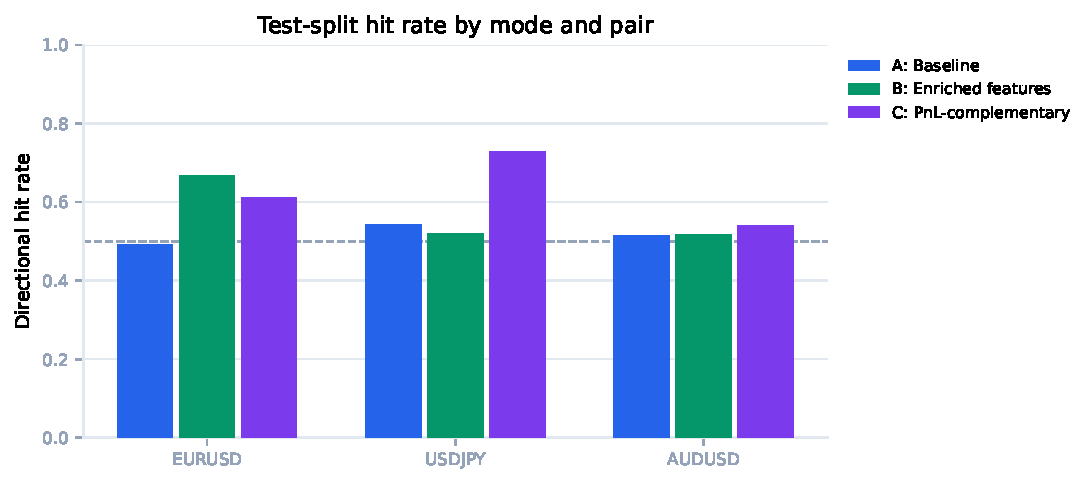
\includegraphics[width=0.85\textwidth]{figures/hit_rate_by_mode.pdf}
\caption{Test-split directional hit rate, all three modes, all three pairs. Dashed line:
random chance (50\%).}
\label{fig:hitratebymode}
\end{figure}

\subsection{Confusion matrix (mode C, test split)}

The full confusion-matrix breakdown for the richest mode, as a representative example of
what every mode/split combination reports:

\begin{center}
\renewcommand{\arraystretch}{1.2}
\small
\begin{tabular}{@{}lccccccccc@{}}
\toprule
Pair & TP & FP & TN & FN & Abst. & Coverage & Precision & Recall & F1 \\
\midrule
EURUSD & 49 & 30 & 9  & 7  & 107 & 47.0\% & 62.0\% & 87.5\% & 0.726 \\
USDJPY & 40 & 6  & 6  & 11 & 139 & 31.2\% & 87.0\% & 78.4\% & 0.825 \\
AUDUSD & 58 & 43 & 14 & 18 & 69  & 65.8\% & 57.4\% & 76.3\% & 0.655 \\
\bottomrule
\end{tabular}
\end{center}

USDJPY combines the highest precision (87.0\%) with the lowest coverage (31.2\%) -- the
neutral band (\S\ref{sec:neutralband}) is abstaining on the majority of USDJPY days and
speaking only when confident, exactly its intended behavior; AUDUSD's higher coverage
(65.8\%) at lower precision reflects the opposite trade-off.

\subsection{Portfolio Sharpe: modulated vs.\ risk-parity baseline}

\begin{center}
\renewcommand{\arraystretch}{1.2}
\resizebox{\textwidth}{!}{%
\begin{tabular}{@{}lcccccc@{}}
\toprule
 & \multicolumn{2}{c}{Train} & \multicolumn{2}{c}{Validation} & \multicolumn{2}{c}{Test} \\
\cmidrule(lr){2-3}\cmidrule(lr){4-5}\cmidrule(lr){6-7}
Mode & Modulated & Risk parity & Modulated & Risk parity & Modulated & Risk parity \\
\midrule
A: Baseline  & 1.701 & 0.040 & \phantom{-}0.125 & -0.359 & -0.153 & 1.764 \\
B: Enriched  & 2.399 & 0.040 & -1.023 & -0.359 & \phantom{-}0.901 & 1.764 \\
C: PnL-mode  & 4.321 & 0.040 & -0.069 & -0.359 & \phantom{-}1.842 & 1.764 \\
\bottomrule
\end{tabular}%
}
\end{center}

(Annualized Sharpe of daily whole-book PnL; risk-parity baseline is identical across modes
within a split by construction -- Eq.~\ref{eq:erc} depends only on realized returns, never
on any model's probabilities.) Train Sharpe rises sharply with mode, most dramatically for
C, whose training objective directly targets exactly this quantity (\S\ref{sec:sharpeobjective}) --
expected, and not by itself evidence of a better model (this is precisely the in-sample
number a Sharpe-trained model is supposed to be able to inflate). The more informative read
is TEST, held out from every training and selection decision: modulated Sharpe improves
monotonically across modes ($-0.153 \to 0.901 \to 1.842$), though it never overtakes the
risk-parity baseline's own test Sharpe ($1.764$) in modes A/B, and only modestly exceeds it
in mode C -- on this single train/val/test partition and single seed, richer features plus
the complementary Sharpe objective move the modulated book from clearly worse than the naive
diversified baseline to roughly on par with it, not to a decisive outperformance.

\begin{figure}[H]
\centering
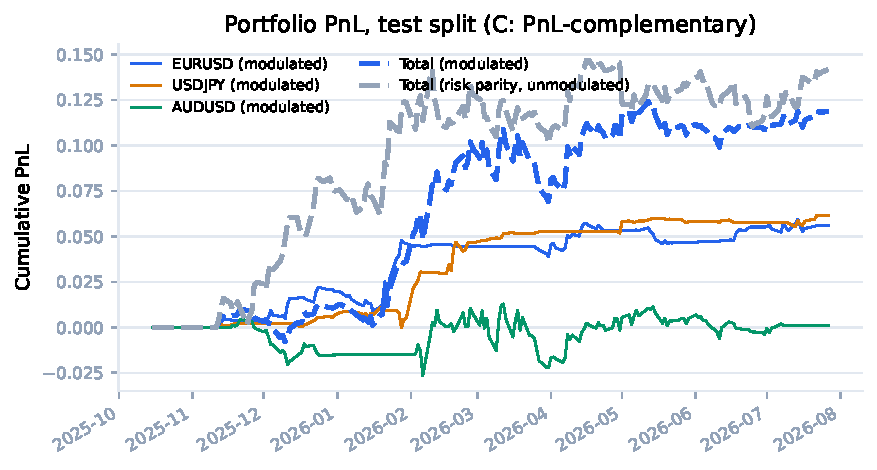
\includegraphics[width=0.85\textwidth]{figures/portfolio_pnl_C_pnl_mode_test.pdf}
\caption{Mode C, test split: cumulative PnL per asset (modulated) and the whole-book total,
modulated versus the unmodulated risk-parity baseline.}
\label{fig:portfoliopnl}
\end{figure}

\begin{center}
\renewcommand{\arraystretch}{1.2}
\small
\begin{tabular}{@{}lccc@{}}
\toprule
Year & Days & Sharpe (modulated) & Sharpe (risk parity) \\
\midrule
2025 & 55  & 1.77 & 4.72 \\
2026 & 147 & 1.99 & 1.06 \\
\bottomrule
\end{tabular}
\end{center}
Mode C, test split, per-calendar-year breakdown (the test window spans a partial 2025 and a
partial 2026) -- exactly the per-year Sharpe table now surfaced live in both the Training and
Evaluation pages. Neither year is a single outlier driving the whole-period number in either
direction.

\subsection{Colored cumulative return and predicted probability (mode C, test, EURUSD)}

\begin{figure}[H]
\centering
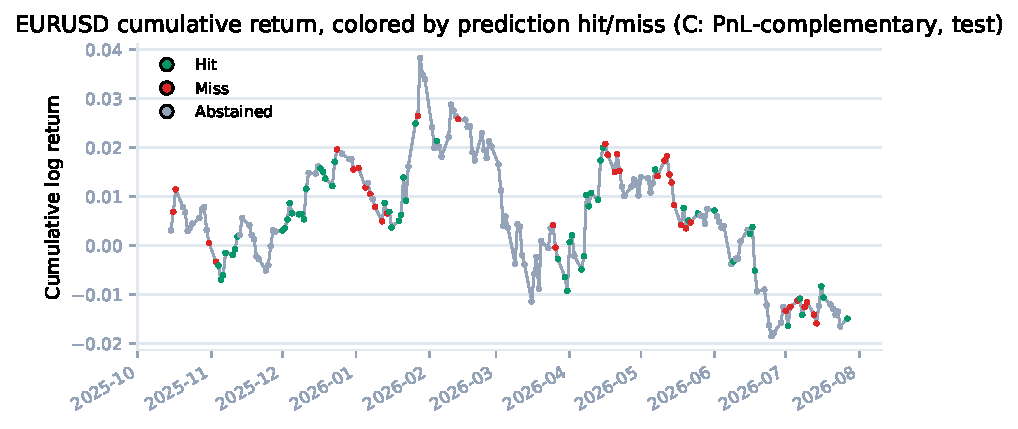
\includegraphics[width=0.8\textwidth]{figures/colored_return_EURUSD_C_pnl_mode.pdf}
\caption{EURUSD's own cumulative (single-day-ahead) log return, test split, mode C -- each
day colored by whether that day's directional call was a hit, a miss, or an abstention
(inside the neutral band).}
\label{fig:coloredreturn}
\end{figure}

\begin{figure}[H]
\centering
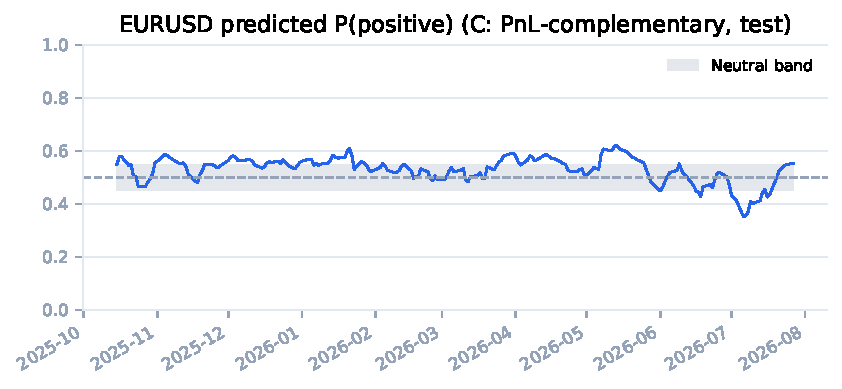
\includegraphics[width=0.8\textwidth]{figures/probability_EURUSD_C_pnl_mode.pdf}
\caption{EURUSD's predicted P(positive), test split, mode C. Shaded band: the neutral band
($\pm 0.05$ around $0.5$) -- probabilities inside it are abstentions, not weak directional
calls.}
\label{fig:probability}
\end{figure}

\begin{figure}[H]
\centering
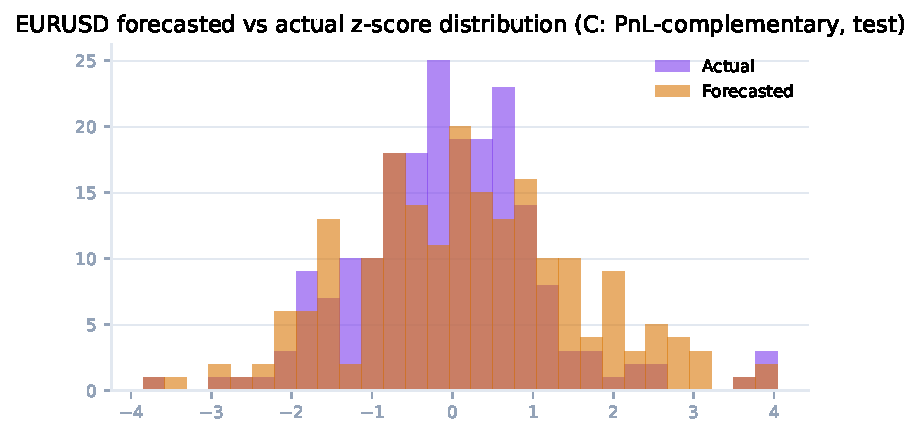
\includegraphics[width=0.72\textwidth]{figures/distribution_EURUSD_C_pnl_mode.pdf}
\caption{EURUSD forecasted (one sample per row from the model's own $N(\mu,\sigma\hat\sigma_{\text{hat}})$)
versus actual realized z-score, test split, mode C -- a distributional calibration check, not
a point-accuracy one.}
\label{fig:distribution}
\end{figure}

\subsection{Honest limitations of this results section}

\begin{rationale}\rationalelabel
This is a \textbf{single seed, single restart, single train/val/test partition}, on three
pairs, over one 8-year history ending at the time of writing -- enough to demonstrate that
every architectural piece described in this document runs correctly end-to-end and produces
internally consistent numbers (e.g.\ hit rate and confusion-matrix coverage/precision agree
exactly; the risk-parity baseline is identical across modes as it must be), but
\textbf{not} enough to claim mode C is statistically better than mode A on this asset
universe. A rigorous claim would need multiple seeds (\code{n\_seeds}$>1$, this system's own
built-in mechanism for exactly this), multiple train/val/test partitions (walk-forward), and
ideally more than three assets. The validation-split reversal for EURUSD between modes A and
B is a concrete illustration of exactly why: a few hundred validation days is not enough to
distinguish "this configuration is worse" from "this seed's validation window happened to be
unfavorable for this configuration".
\end{rationale}

\newpage


% =============================================================================
\section{Configuration Reference}
\label{sec:config}
% =============================================================================

Every key below lives in \code{DEFAULT\_CONFIG} (\texttt{models/portfolio\_lstm.py:1643--1767});
a JSON config passed to \texttt{main.py} only needs to specify keys that differ from these
defaults. \code{"pairs"} is the only key with no default.

\begin{center}
\renewcommand{\arraystretch}{1.2}
\small
\begin{longtable}{@{}p{3.4cm}p{2.0cm}p{9.4cm}@{}}
\toprule
\textbf{Key} & \textbf{Default} & \textbf{Meaning} \\
\midrule
\endhead
\code{pairs} & \emph{required} & FX pairs, e.g.\ \code{["EURUSD","USDJPY","AUDUSD"]} \\
\code{lookback} & 30 & Days per input window ($L$) \\
\code{years} & 8 & Years of history fetched \\
\code{train\_frac} / \code{test\_frac} & 0.8 / 0.1 & Chronological split fractions (\S\ref{sec:split}) \\
\code{direction\_horizon} & 5 & Forward days the z-score label looks ($H_d$) \\
\code{rolling\_stats\_window} & 20 & Trailing window for vol/skew/kurt + label normalization ($W_r$) \\
\code{features} & \code{[log\_return,vol,skew,kurt]} & Selected input channels (\S\ref{sec:features}) \\
\code{cma\_windows} / \code{bandpass\_windows} & \code{[]} / \code{[]} & (short, long) window pairs for \code{"cma"}/\code{"bandpass"} \\
\code{bandpass\_order} & 3 & Butterworth filter order (Eq.~\ref{eq:lfilter}) \\
\code{cross\_pairs} & \code{\{\}} & Per-pair opt-in cross-asset input widening (\S\ref{sec:crosspairs}) \\
\code{hidden\_size} & 16 & \texttt{AssetLSTM} hidden width $H$ \\
\code{num\_layers} & 1 & LSTM layers (see \S\ref{sec:numericalissues} before raising with \code{device="mps"}) \\
\code{dropout} & 0.1 & Dropout, LSTM + attention \\
\code{n\_attn\_heads} & 4 & Causal self-attention heads $K$ \\
\code{epochs} & 300 & Training epochs \\
\code{lr} / \code{weight\_decay} & $10^{-3}$ / $10^{-4}$ & Adam hyperparameters (per-asset instance) \\
\code{bce\_weight} & 1.0 & $\lambda_{\text{bce}}$ (Eq.~\ref{eq:bce}); accepts a list to sweep \\
\code{sharpe\_weight} & 0.0 & Optional joint Sharpe phase weight (\S\ref{sec:sharpeobjective}); 0 disables \\
\code{sharpe\_window} & 20 & Rolling window $W_s$ for Eq.~\ref{eq:rollingsharpe} \\
\code{neutral\_band} & 0.05 & Abstention half-width (\S\ref{sec:neutralband}) \\
\code{target\_vol} & 0.10 & Annualized target volatility (Eq.~\ref{eq:voltarget}) \\
\code{n\_seeds} & 1 & Independent restarts, best validation log-loss wins \\
\code{device} & \code{"auto"} & \code{"auto"}/\code{"cpu"}/\code{"mps"}/\code{"cuda"} \\
\code{save\_db} & \code{False} & Also persist to \code{quant.model\_registry} \\
\bottomrule
\end{longtable}
\end{center}

% =============================================================================
\section{Summary of Architectural Decisions}
\label{sec:summary}
% =============================================================================

\begin{center}
\renewcommand{\arraystretch}{1.3}
\small
\begin{longtable}{@{}p{4.0cm}p{5.6cm}p{5.6cm}@{}}
\toprule
\textbf{Decision} & \textbf{What it replaced / alternative} & \textbf{Why} \\
\midrule
\endhead
Fully independent per-asset training & One shared optimizer over every asset's parameters & Isolates each asset's own gradient signal; verified byte-identical solo-vs-paired (\S\ref{sec:training}) \\
\code{cross\_pairs}, default off & Unconditional full cross-asset mixing & Opt-in, per-pair, explicit -- no way to dial back an always-on design \\
Causal self-attention over LSTM output & LSTM's final hidden state alone & Avoids the fixed-size bottleneck of $h_n[-1]$ for longer lookbacks; verified causal via perturbation test \\
Gaussian NLL + direction BCE & Plain regression (MSE/Huber) & Anti-collapse: BCE forces $\mu$ to spread per-sample sign, not settle on the unconditional mean \\
Neutral band as pure postprocessing & Baked into training/reporting & Enables live, client-side band recomputation with no retraining \\
Risk parity, not equal weight & Naive $1/N$ weighting & Accounts for correlation in the risk contribution, not just variance \\
Smooth product, not signal, before vol-scaling & Smoothing the raw signal alone & Matches the actual deployed strategy exactly (Reading B, \S\ref{sec:sharpeobjective}) \\
Butterworth band-pass via \code{lfilter} & \code{filtfilt} (the "usual" way) & \code{filtfilt} is non-causal -- leaks future returns \\
Precomputed risk parity for the Sharpe objective & Solving ERC inside the training loop & The ERC solve isn't differentiable (external SLSQP call); it's also DATA-ONLY, so precomputing once is exact, not an approximation \\
\code{\_assert\_finite\_grad} safety net & Silent NaN propagation & Turns a wasted 300-epoch run into an immediate, actionable error \\
\bottomrule
\end{longtable}
\end{center}

\end{document}




